\documentclass{article}
\usepackage[utf8]{inputenc}

\title{Literature Review of Machine Learning Methods}
\author{Jonathan Gillett}
\date{July 2015}

\usepackage{natbib}
\usepackage{graphicx}
\usepackage{url}
\usepackage{setspace}
\usepackage{floatrow}

\newcommand{\bold}[1]{\textbf{#1}}

\begin{document}

\maketitle

\begin{abstract}

Machine Learning methods have numerous applications in scientific fields and in highly commercialized industries. The ability to organize data into sensible groupings that can be more easily understood and analyzed is fundamental to understanding the vast amount of data available. The focus of this literature review is on Machine Learning methods for data clustering and dimensionality reduction and how these methods are improved using intelligent methods.

\end{abstract}


\section{Introduction}

Machine Learning is a branch of Computer Science that has since evolved from the study of pattern recognition and computational theory into a highly diverse and widely applied area of research. This evolution has begun to empower society to take advantage of the almost limitless amount of data that has become available\cite{lohr2012age, mohri2012foundations}.

Machine Learning focuses on the creation of algorithms, often rooted in artificial intelligence methods; in order to learn from, model, and make predictions based on data.\cite{dietterich2002machine}. These algorithms frequently involve the analysis and understanding of large data sets, often referred to as ``Big Data'', which are seemingly insurmountable using traditional statistical methods\cite{lohr2012age}. For example, in 2007 there was approximately 281 exabytes of data consumed on the Internet, and by 2011 this amount had increased tenfold\cite{jain2010}. Most of this data is stored digitally in electronic media, thus providing huge potential for the development of automatic data analysis, classification, and retrieval techniques.

The increase in the sheer volume and the variety of data requires advances in methodology to automatically understand, process, and summarize the data. As such, this has created a huge demand for Machine Learning techniques, which are applied to the data for performing clustering analysis, dimensionality reduction, and modelling to better understand and predict trends. Clustering analysis involves algorithms for grouping or clustering objects according to measured or perceived intrinsic characteristics or similarity; making it possible to find patterns which would otherwise be indistinguishable\cite{jain2010}. Furthermore, dimensionality reduction is also an essential step in Machine Learning, and is used to reduce the negative affects of the ``curse of dimensionality'', which often arises when an algorithm does not scale well to high-dimensional data, requiring time or memory that increases exponentially based on the dimensions of the data\cite{domingos2012few}. 

Given the importance of Machine Learning techniques to the scientific community it is the purpose of this review paper to provide an overview of clustering and dimensionality reduction algorithms used in Machine Learning, with a focus on the applications of intelligent methods to improve their accuracy and robustness.







\section{Review of Clustering Methods}

Clustering, also known as cluster analysis, is essential to discovering the natural groupings of a set of patterns, points, or objects within the data. All clustering methods can be described as follows: 
Given a representation of $N$ objects, find $K$ groups based on a measure of similarity such that the similarities between objects in the same group are high while the similarities between objects in different groups are low\cite{jain2010}.

As a result of the similarity criteria for clustering, it can be expected that clustering is a subjective entity that often is in the eye of the beholder and whose significance and interpretation requires domain knowledge. As a result of the requirement for domain knowledge, it has resulted in thousands of clustering algorithms being published for use, and that continue to appear\cite{jain2010}. The rapid increase in clustering algorithms has created a need for an underlying robust clustering method that uses intelligent methods to encapsulate some of the domain knowledge of the expert without requiring a new algorithm. The vast amount of literature citing the use of clustering algorithms speaks to the importance of clustering in data analysis. 

The intent of this section is to provide a review of K-means clustering methods, discuss the development and refinements of clustering algorithms, and lastly to point out some of the emerging and useful research directions that utilize intelligent methods to improve the accuracy and robustness of clustering.




\subsection{\emph{Some Methods for Classification and Analysis of Multivariate Observations} \& \emph{Least Squares Quantization in PCM}}

K-means has a rich and diverse history as it was independently discovered in multiple scientific fields prior to it's formalization and independent publication by Lloyd (published in 1982)\cite{lloyd1982least} and MacQueen (published in 1967)\cite{macqueen1967some}. Despite the fact that K-means was first proposed over 50 years ago, it is still one of the most widely used algorithms for clustering\cite{jain2010}.

In K-means the data is clustered by first determining a set of centroid points. The algorithm then finds a partition, such that the squared error between the empirical mean of a cluster and the centroid points in the cluster is minimized\cite{macqueen1967some, lloyd1982least}.

As outlined independently by MacQueen and Lloyd in their publications of the K-means clustering algorithm, it can be formally described in mathematical terms as follows.

Let $X = {x_i}, i = 1, \ldots, n$ be the set of $n$ $d$-dimensional points to be clustered into a set of $K$ clusters, $C = {c_k, k = 1, \ldots, K}$. K-means algorithm finds a partition such that the squared error between the empirical mean of a cluster and the points in the cluster is minimized. Let $\mu_k$ be the mean of the cluster $c_k$, the squared error between $\mu_k$ and $c_k$ is defined as follows.

\begin{equation}
J(c_k) = \sum_{x_i \in c_k}^{} \|x_i - \mu_x\|^{2}
\label{eq:kmeans1}
\end{equation}

Where the optimization criteria of K-means is to minimize the sum of the squared error over all K clusters.

\begin{equation}
J(C) = \sum_{k = 1}^{K} \sum_{x_i \in c_k}^{} \|x_i - \mu_x\|^{2}
\label{eq:kmeans2}
\end{equation}

\subsubsection{Reflections}

The main reasons for the continued popularity of K-means is due to the ease of implementation, simplicity, and efficiency\cite{jain2010}. The subsequent 50 years of development in clustering algorithms have been based on the equations \ref{eq:kmeans1} and \ref{eq:kmeans2} for K-means. 

While K-means has been the most popular clustering algorithm, the original algorithm does not take into consideration any information about the problem domain; limiting it's accuracy and robustness in comparison to subsequent improvements\cite{jain2010}. 

Lastly, it is important to note that the K-means optimization criteria for the final clustering, as described in equation \ref{eq:kmeans2}, which minimizes the sum of the squared error over all $K$ clusters is \bold{NP-HARD}\cite{drineas2004clustering}.








\subsection{\emph{The Uniqueness of a Good Optimum for K-Means}}

In this paper the author, Meila, focused on addressing the most critical issue in K-means; that the optimization criteria for the final clustering is \bold{NP-HARD}. The paper provides proofs that it is possible to find a ``good'' clustering $C$ of a data set that is not far from the optimal, by measuring the ``goodness'' of the distortion of K-means clustering.

It is significant as the paper proves the spectral bounds on the distance $d(C, C^{opt})$, where $C$ is a cluster and $C^{opt}$ the optimal, that it is possible to find a ``good'' clustering of $C$ without having to perform the \bold{NP-HARD} computation required to find the best clustering\cite{meilua2006uniqueness}. Thus, by using a measure of ``goodness'' a unique and compact cluster of near-optimal clusterings can be found without needing to perform the computationally expensive \bold{NP-HARD} operation\cite{meilua2006uniqueness}.


\subsubsection{Reflections}

This paper is significant in that it provides the first proven method of reducing the daunting \bold{NP-HARD} complexity of the K-means clustering method; which is often amplified given the sheer magnitude of the data being analyzed in most Big Data applications of Machine Learning techniques.

By providing a proven method for finding a suitable clustering that is a ``good'' fit, without requiring evaluating all possible clusters, the results of this paper made the continued widespread adoption of K-means even more applicable given the increased performance that it can have when applied to increasingly large data sets.




\subsection{\emph{Estimating the Number of Clusters in a Data Set via the Gap Statistic}}

The K-means algorithm requires three user-specified parameters: number of clusters $K$, cluster centroids initialization, and a distance metric\cite{tibshirani2001estimating}. These are all dependent on the domain knowledge of the expert, with the most critical choice parameter being $K$, the number of clusters.

While there is no perfect mathematical criterion that exists, there are a number of heuristic approaches available for choosing $K$. Typically, K-means is run independently for different values of K and the partition that appears the most meaningful to the domain expert is then selected. This poses a problem as the different initializations can often lead to vastly different final clustering because K-means only converges to local minimal\cite{tibshirani2001estimating}.

In order to mitigate this time-consuming and computationally expensive process, Tibshirani, et al. introduced a method of estimating the number of clusters in a group, referred to as the ``gap statistic'', to limit the requirement of domain knowledge\cite{tibshirani2001estimating}. As a result, this enhancement greatly increased the robustness of K-means, in addition to enhancing the intelligence of the ``unsupervised'' learning of K-means, requiring less domain knowledge to create the optimal results.


\subsubsection{Reflections}

The method of the ``gap statistic'' introduced by Tibshirani, et al. made it possible to perform K-means without requiring domain knowledge about the number of clusters in the data. However, the remaining parameters essential to K-means: the cluster centroids initializations, and distance metrics still require domain knowledge.

The use of additional intelligent methods such as evolutionary computation, Genetic Algorithm (GA), would make it possible to make K-means purely unsupervised, thus relying on the optimization abilities of GA, rather than requiring a domain expert to specify parameters. The GA could be used to enhance the ``gap statistic'' by optimizing the remaining parameters of the k-means clustering.




\subsection{\emph{K-means Clustering of Proportional Data using L1 Distance}}

The third parameter required for K-means is the distance metric, most frequently the Euclidean distance is used as the metric for computing the distance between points and cluster centroids\cite{kashima2008k}. Thus, as a result, K-means gravitates towards finding spherical or ball-shaped clusters in data, however this is not always the desired outcome, especially for higher-dimensional data. 

To address this issue, Kashima et al. introduced the application a new distance metric for K-means known as $L1$, or more commonly referred to as \emph{Manhattan distance}. The $L1$ distance, is simply the sum of the absolute differences of their Cartesian coordinates projected onto the determined coordinate with fixed step size\cite{kashima2008k}. More formally, the $L1$ distance can be described as follows where $p, q$ are vectors on a fixed Cartesian coordinate system.

\begin{equation}
d_1(p, q) = \|p - q\|_1 = \sum_{i = 1}^{n} |p_i - q_i|
\label{eq:l1}
\end{equation}

Where $(p, q)$ are vectors defined as follows.

\begin{equation}
p = (p_1, p_2, \ldots, p_n) \mbox{ \bold{ and } } q = (q_1, q_2, \ldots, q_n)
\label{eq:l1vec}
\end{equation}



\subsubsection{Reflections}

The research done by Kashima et al. improves the third parameter of K-means, the distance comparison metric, by using the $L1$ distance method instead of the default Euclidean distance, this is yet another improvement to K-means in addition to the application of the ``gap statistic'' introduced by Tibshirani, et al.\cite{tibshirani2001estimating}.

However, both the ``gap statistic'' and the $L1$ distance metric introduced by Tibshirani, et al. and Kashima et al.\cite{tibshirani2001estimating, kashima2008k} lack the application of soft methods for determining the distances and thus membership of data within clusters.

There is much potential for future applications of clustering methods that use fuzzy logic and set theory for the distance metrics and clustering memberships, to categorize clusters rather than relying solely on a crisp membership within clusters based on the distance.




\subsection{\emph{Fast Accurate Fuzzy Clustering through Data Reduction}}

One of the major improvements to the original K-means method published independently by Lloyd and MacQueen\cite{lloyd1982least, macqueen1967some} is the fuzzy C-means method of clustering. As it's name implies, fuzzy C-means applies the intelligent soft computing methods of fuzzy logic and set theory to provide fuzzy membership within clusters rather than the traditional crisp sets that are used to denote membership within a cluster.

Fuzzy C-means was first proposed by Dunn in 1973\cite{dunn1973fuzzy} and later improved by Bezdek in 1984\cite{bezdek1984fcm}, and extended the robustness of K-means by making it possible for each data point to be a member of multiple clusters with a membership value for each (soft assignment). Despite the benefits of the soft assignments of fuzzy C-means, it's application was limited due to the performance overhead until recently when Eschrich et al. published their method on performing fast fuzzy C-means through data reduction\cite{eschrich2003fast}.

In their paper Eschrich et al. provide a method of improving the performance of fuzzy C-means with their algorithm, brFCM, which performs a reduction and aggregation of similar examples and then uses a weighted exemplar in the clustering process\cite{eschrich2003fast}. The brFCM algorithm performs quantization of the data, reducing it from a continuous data type to one that has an acceptable level of quantization at the expense of a loss in precision. Following the quantization, the data is aggregated to combine identical feature vectors into a single weighted exemplar. The quantization then performs fine-grained binning of the data making it easier to find identical feature vectors for the aggregation process\cite{eschrich2003fast}.


\subsubsection{Reflections}

While the performance of the method demonstrated by Eschrich et al. provided a 59 to 290 improvement over a traditional implementation of fuzzy C-means using brFCM\cite{eschrich2003fast}, the performance is still not optimal for clustering of Big Data due to the overhead of the fuzzy set operations\cite{jain2010}.

However, the use of brFCM for fuzzy C-means demonstrably provides more optimal clustering than the default operations and the intelligent methods of fuzzy set theory make it possible to have accurate clusters without having to rely on ``gap statistics''  to find the optimal number of clusters\cite{tibshirani2001estimating}.








\section{Review of Dimensionality Reduction Methods}

Dimensionality reduction is essential in Machine Learning to reduce the negative affects of the ``curse of dimensionality'', which often arises when an algorithm does not scale well to high-dimensional data, requiring time or memory that increases exponentially based on the dimensions of the data\cite{domingos2012few}. Dimensionality reduction is used to reduce the number of dimensions of the data, making it more easily comprehensible as a reduced number of components which encapsulate the majority of the variance in the data.

Dimensionality is a quintessential operations in Machine Learning, with numerous applications in other fields. The most widely used methods in Machine Learning is Principal Component Analysis (PCA)\cite{jain2010, domingos2012few, dietterich2002machine}, but more recently groundbreaking research has been done by leading researchers in Deep Learning to create a more intelligent algorithm for dimensionality reduction known as t-distributed Stochastic Neighbor Embedding (t-SNE).

The intent of this section is to provide a literature review of the most widely used dimensionality reduction methods, PCA and t-SNE, and to discuss the latest research in this area.




\subsection{\emph{Principal Component Analysis}}

Dimensionality reduction is an essential operation in Machine Learning, PCA provides a method of reducing the dimensionality of higher dimensional data into it's ``principal components''. The essential concept of PCA is a method to transforms a number of possibly correlated variables into a smaller number of variables, which are called principal components\cite{richardson2009principal, abdi2010principal}.

The principal components make it possible to perform a visual (in 1 - 3 dimensions) and even quantitative examination (for higher dimensions) of the reduced dimensional data set. This allows the domain expert to spot trends, patterns and outliers in the data, far more easily than would have been possible without performing the principal component analysis\cite{richardson2009principal}.

In computing the principal components the first task of PCA is to identify a new set of orthogonal coordinate axes through the data, this is achieved by finding the direction of maximal variance through the coordinates in the $N$ dimensional space\cite{richardson2009principal}. These coordinates are then used to project the $N$-dimensional data onto a $K$-dimensional linear subspace that minimizes the \emph{reconstruction error}, which is the sum of the squared $L_2$-distances between the original and projected data. The resultant projection of this operation captures the most variance in the data within the orthogonal principal components of the linear subspace\cite{richardson2009principal, abdi2010principal, mohri2012foundations}.  
Following the selecting of the initial principal component such that it meets this criteria, the PCA method then proceeds to obtain further principal coordinate (axis) which are both orthogonal to the other previously selected principal components, and are the next best direction maximizing the variance in the data, chosen from directions which are orthogonal to the first principal component\cite{richardson2009principal, mohri2012foundations}.


\subsubsection{Reflections}

PCA is often referred to as one of the most important results to come out of the field of applied linear algebra\cite{richardson2009principal}, and for good reason. PCA has proven to be very versatile, and is one of the oldest and most popular techniques used in dimensionality reduction for multivariate analysis\cite{abdi2010principal}. With PCA it is possible to reduce a seemingly incomprehensible multivariate problem into one that can have the majority of the variance explained by only a few principal components using only common linear algebraic operations\cite{richardson2009principal}.

Despite the longevity and popularity of PCA, it does not incorporate any intelligent methods, such as evolutionary computation, or fuzzy logic in order to improve it's robustness and provide soft selection of principal components. However, as will be discussed in the proceeding sections, \emph{t-SNE} has proven to be a strong contender to PCA with it's inception rooted in Deep Learning.




\subsection{\emph{A General Framework for Increasing the Robustness of PCA-based Correlation Clustering Algorithms}}

Expanding upon the long history and popular adoption of PCA, Kriegel, et al. focused on making PCA more robust to outliers in the data. By it's nature PCA is rather sensitive to outliers, if a small fraction of these points do not correspond to the correct correlation of the cluster, the algorithms are usually misled or even fail to detect the correct results\cite{kriegel2008general}.

Kriegel, et al. evaluated the influence of outliers on PCA and proposed a general framework for increasing the robustness of PCA, and found in many cases when performing PCA that if the correct subspace of the corresponding cluster contains noise the subspace determination process will be misled\cite{kriegel2008general}.

In order to address the influence of outliers and noise on PCA Kriegel, et al. proposed a weighting function which significantly reduces the negative impact of outliers on PCA.  First, a weighting function is applied to the points when computing the covariance matrix, this is done in order to weight points that are potential outliers, or noisy, lower than points that are potential cluster members. After the weighting is applied a method for selecting a suitable number of neighbors for each cluster member or cluster is applied by micro-adjusting the parameters to avoid sudden drops in the explained variance and choosing significantly different parameters for points in the data set\cite{kriegel2008general}.


\subsubsection{Reflections}

Almost all correlation clustering algorithms suffer from an arbitrary selection of points in the local neighborhood of cluster members, and are heavily dependent on the initial choice made. The process of selecting the correct cluster members from which the subspace of a cluster is determined by applying PCA often has a significant influence on the amount of outliers in the data.

Kriegel, et al. focused on not solving the problem of making more suitable selections of cluster members, but instead focused on trying to lessen the negative influence of outliers and noisy data on PCA. The weighting and micro-adjusting method provides a useful, but unfortunately non-intelligent method of improving the robustness of PCA. It is interesting to note what potential benefits their method would have if it was enhanced by fuzzy logic and set theory to make the selection of cluster members soft rather than crisp.


\subsection{\emph{Visualizing Data Using t-SNE}}

One of the most significant advances in dimensionality reduction since the inception of PCA has been t-distributed Stochastic Neighbor Embedding (t-SNE) created by leading Machine Learning researchers, Van der Maaten and Hinton. t-SNE makes it possible to visualize high-dimensional data giving each data point a location in a two or three-dimensional map, making it much easier to optimize and produces significantly better visualizations by reducing the tendency to crowd points together in the center of the map\cite{van2008visualizing}.

The origin of t-SNE is one born out of dissatisfaction, after investigating all of the leading methods of non-linear dimensionality reduction (e.g. PCA) that aim to preserve the local structure, Van der Maaten and Hinton were dissatisfied with the weak performance on real high-dimensional data\cite{van2008visualizing}. Motivated to come up with a revolutionary new method of dimensionality reduction, t-SNE was created and tested against many other leading dimensionality reduction algorithms using real high-dimensional data. On almost all of the data sets tested by Van der Maaten and Hinton the visualizations produced by t-SNE were significantly better, providing a much clearer identification of clusters.

% FIGURES
\begin{figure}[H]
\centering
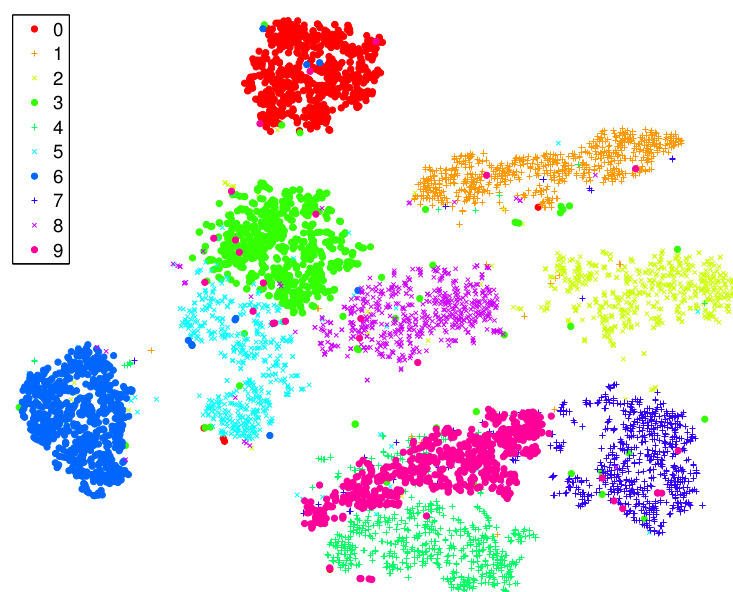
\includegraphics[width=0.62\textwidth]{figures/tsne-cluster}
\caption{Clustering of 6,000 handwritten digits from MNIST data set using t-SNE\cite{van2008visualizing}}.
\label{fig:tsne-cluster}
\end{figure}


\begin{figure}[H]
\centering
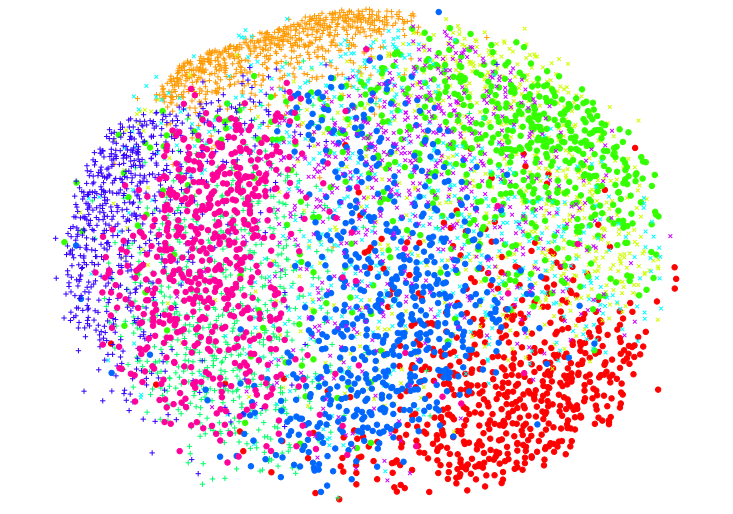
\includegraphics[width=0.62\textwidth]{figures/other-cluster}
\caption{Clustering of 6,000 handwritten digits from MNIST data set using linear dimensionality reduction (e.g. PCA)\cite{van2008visualizing}}.
\label{fig:other-cluster}
\end{figure}

The failings of linear techniques such as PCA for high-dimensional data, is that they focus on keeping the low-dimensional representations of dissimilar data points far apart. This is problematic as for very high dimensional that lies on or near a low-dimensional, non-linear manifold it is usually more important to keep the low-dimensional representations of very similar data points close together\cite{van2008visualizing}. This is something that is not typically possible with a linear mapping such as used by PCA.

Stochastic Neighbor Embedding (SNE), the basis of t-SNE, is based on the concept of converting high-dimensional Euclidean distances between data points into conditional probabilities that represent similarities. The following equation describes the similarity of data point $x_j$ to data point $x_i$ as the conditional probability, $p_{j|i}$, that $x_i$ would pick $x_j$ as its neighbor if the neighbours were picked proportionally based on their probability density under a Gaussian distribution centered at $x_i$\cite{van2008visualizing}.

Mathematically, this conditional probability $P_{j|i}$ used by SNE is given as follows, where $\sigma_{i}$ is the variance of the Gaussian that is centered on the data point $x_i$.

\begin{equation}
P_{j|i} = \frac{exp(-\|x_i - x_j\|^2 / 2\sigma_{i}^2)}{\sum_{k \ne i}^{} exp(-\|x_i - x_k\|^2 / 2\sigma_{i}^2)}
\label{eq:tsne}
\end{equation}

SNE, performs this calculation to determine the pairwise data point similarities, which are the two conditional probabilities  $P_{j|i}$ and $Q_{j|i}$. Using the conditional probability calculations for the pairwise similarities, SNE aims to find a low-dimensional data representation that minimizes the mismatch between $P_{j|i}$ and $Q_{j|i}$.

Using this method SNE constructs reasonably good visualizations, however it is hampered by a cost function that is difficult to optimize and by a problem referred to by Van der Maaten and Hinton to as the ``crowding problem''\cite{van2008visualizing}. t-SNE alleviates these problems by using a unique cost function that differs from SNE in two ways. First the t-SNE cost function uses a symmetrized version of the SNE cost function with simpler gradient calculations. The second and most significant improvement is that t-SNE uses a Student-t distribution, rather than the Gaussian distribution shown in equation \ref{eq:tsne}, to compute the similarity between two points in the low-dimensional space.


\subsubsection{Reflections}

Despite the drastic improvement in the clustering results and accuracy for t-SNE it has severely limiting computational and memory complexities that are quadratic in the number of data points analyzed\cite{van2008visualizing}. While t-SNE performed exceedingly well in comparison to existing methods this limiting computational and memory complexity makes it infeasible to apply the standard version of t-SNE to data sets that contain many more than approximately 10,000 points\cite{van2008visualizing}.

Given this limitation it is unlikely that t-SNE will find greater acceptance with real world data, as Machine Learning methods are being applied to increasingly larger and larger data sets every year\cite{lohr2012age}. Perhaps there is still the potential for t-SNE to find greater application if further improvements can be made to address it's computational and memory complexities, but for now it is likely that the existing methods of K-means and PCA will continue to be used.





\section{Conclusion}

The numerous applications for Machine Learning are obvious, the importance of creating robust and accurate algorithms for performing clustering and dimensionality reduction are critical to understanding and analyzing the ever-increasing amount of information at our disposal. In this review paper we compiled a thorough list of the fundamental techniques and algorithms for the most widely used methods of clustering and dimensionality reduction, K-means and PCA.

After laying the foundation for the two most common methods, we then provided a thorough review of each of the latest improvements that have been made to these algorithms. In the first section for clustering algorithms, the paper \emph{The Uniqueness of a Good Optimum for K-Means}, by Meila, provided a value performance enhancement to K-means making it possible to find a ``good'' clustering that is not far from the optimal, reducing the daunting NP-HARD complexity of K-means for finding the optimal\cite{meilua2006uniqueness}. In \emph{Estimating the Number of Clusters in a Data Set via the Gap Statistic}, Tibshirani provided a method to enhance the intelligence required to execute K-means, estimating the number of clusters using the ``gap statistic'', to limit the requirement of domain knowledge for the number of clusters\cite{tibshirani2001estimating}. Lastly, the most significant paper, \emph{Fast Accurate Fuzzy Clustering through Data Reduction}, by Eschrich et al. provided an innovative method for improving the performance of fuzzy C-means with their algorithm, brFCM. Where, fuzzy C-means applies  the intelligent soft computing methods of fuzzy logic and set theory to provide fuzzy membership within clusters rather than the traditional crisp sets\cite{eschrich2003fast}.

Lastly, following a literature review of clustering methods we provided a thorough review of dimensionality reduction, giving an explanation of the most commonly used method, Principal Component Analysis (PCA). While PCA is one of the oldest and most popular techniques and has proven to be very versatile for dimensionality reduction, there have been no major advances in dimensionality reduction until very recently. Dissatisfied with the poor results of existing methods on real data, leading Machine Learning researchers, Van der Maaten and Hinton, created the revolutionary t-distributed Stochastic Neighbor Embedding (t-SNE) algorithm. t-SNE provided a drastic improvement in the clustering results and accuracy for but unfortunately is severely limited due to the rapid increase in the computational and memory complexity as the number of data points analyzed increase, making it infeasible for very large data sets\cite{van2008visualizing}.

In conclusion, it is significant to note the longevity of the K-means clustering and PCA dimensionality reduction algorithms, after nearly 50 years, these algorithms are still widely utilized for solving real-world problems and continue to be improved by leading Machine Learning experts. We feel that their is still much potential to improve these methods further or to create new algorithms, as demonstrated by Van der Maaten and Hinton with t-SNE, that utilize intelligent methods to further improve the robustness and accuracy of these critical Machine Learning algorithms.




\bibliographystyle{plain}
\bibliography{references}
\end{document}
